\section{Implementation and Performance}
\label{sec:implementation}
% We present ARLayout, a mobile tool that provides a re-layout experience in usage scenarios with AR.
% We begin by describing a generic workflow in usage scenarios. Then, we summarize the implementation points involved based on this workflow, combined with the experimental usage scenarios, and we introduce the design details of each section below.

An implementation overview of the implementation workflow
and the details are described in this section.


%\subsection{Implementation}
%
%\textit{ARLayout} is based on C/S architecture
%that allows users to take photos/record videos in a cluttered environment
%using a mobile device such as iPad or other tablets.
%% The remote server processes the images in real-time, calculates the corresponding data feedback, and displays them by ARLayout.
%We tried \textit{ARLayout} in library, coffee shop, and cosmetics shop,
%three usage scenarios, where the objects will be
%re-grouped and re-ranked in AR space, and generate various augmented visual presentations.


\begin{figure}[htp]
%\setlength{\abovecaptionskip}{0.05cm}
%\setlength{\belowcaptionskip}{-0.4cm}
    \centering
    \includegraphics[width=\linewidth]{images/implementation_ocr.eps}
    \caption{
        % These images show the difficulties of traditional OCR and the corresponding improvements.
        The difficulties of traditional OCR and the corresponding improvements.
        (a): Books are slanted.
        (b): The texts of books are calibrated first.
        (c) and (d): The difference in the arrangement of text between Chinese and English books.
        % Artistic fonts occurs in (e).
        % The non-uniform width and the existence of special deformation of the font,
        %sometimes affect the accuracy of recognition. Therefore, when recognition is difficult,
        %we try to infer the content of the book from the rest of the text in the spine.
        % (f) and (g) define the reference regions required for a custom template.
        % Reference Fields are identified in (f) and Identification Areas are identified in (g).
    }
    \label{fig:implementation_ocr}
\end{figure}


\begin{figure}[htp]
%\setlength{\abovecaptionskip}{0.05cm}
%\setlength{\belowcaptionskip}{-0.4cm}
    % \centering
    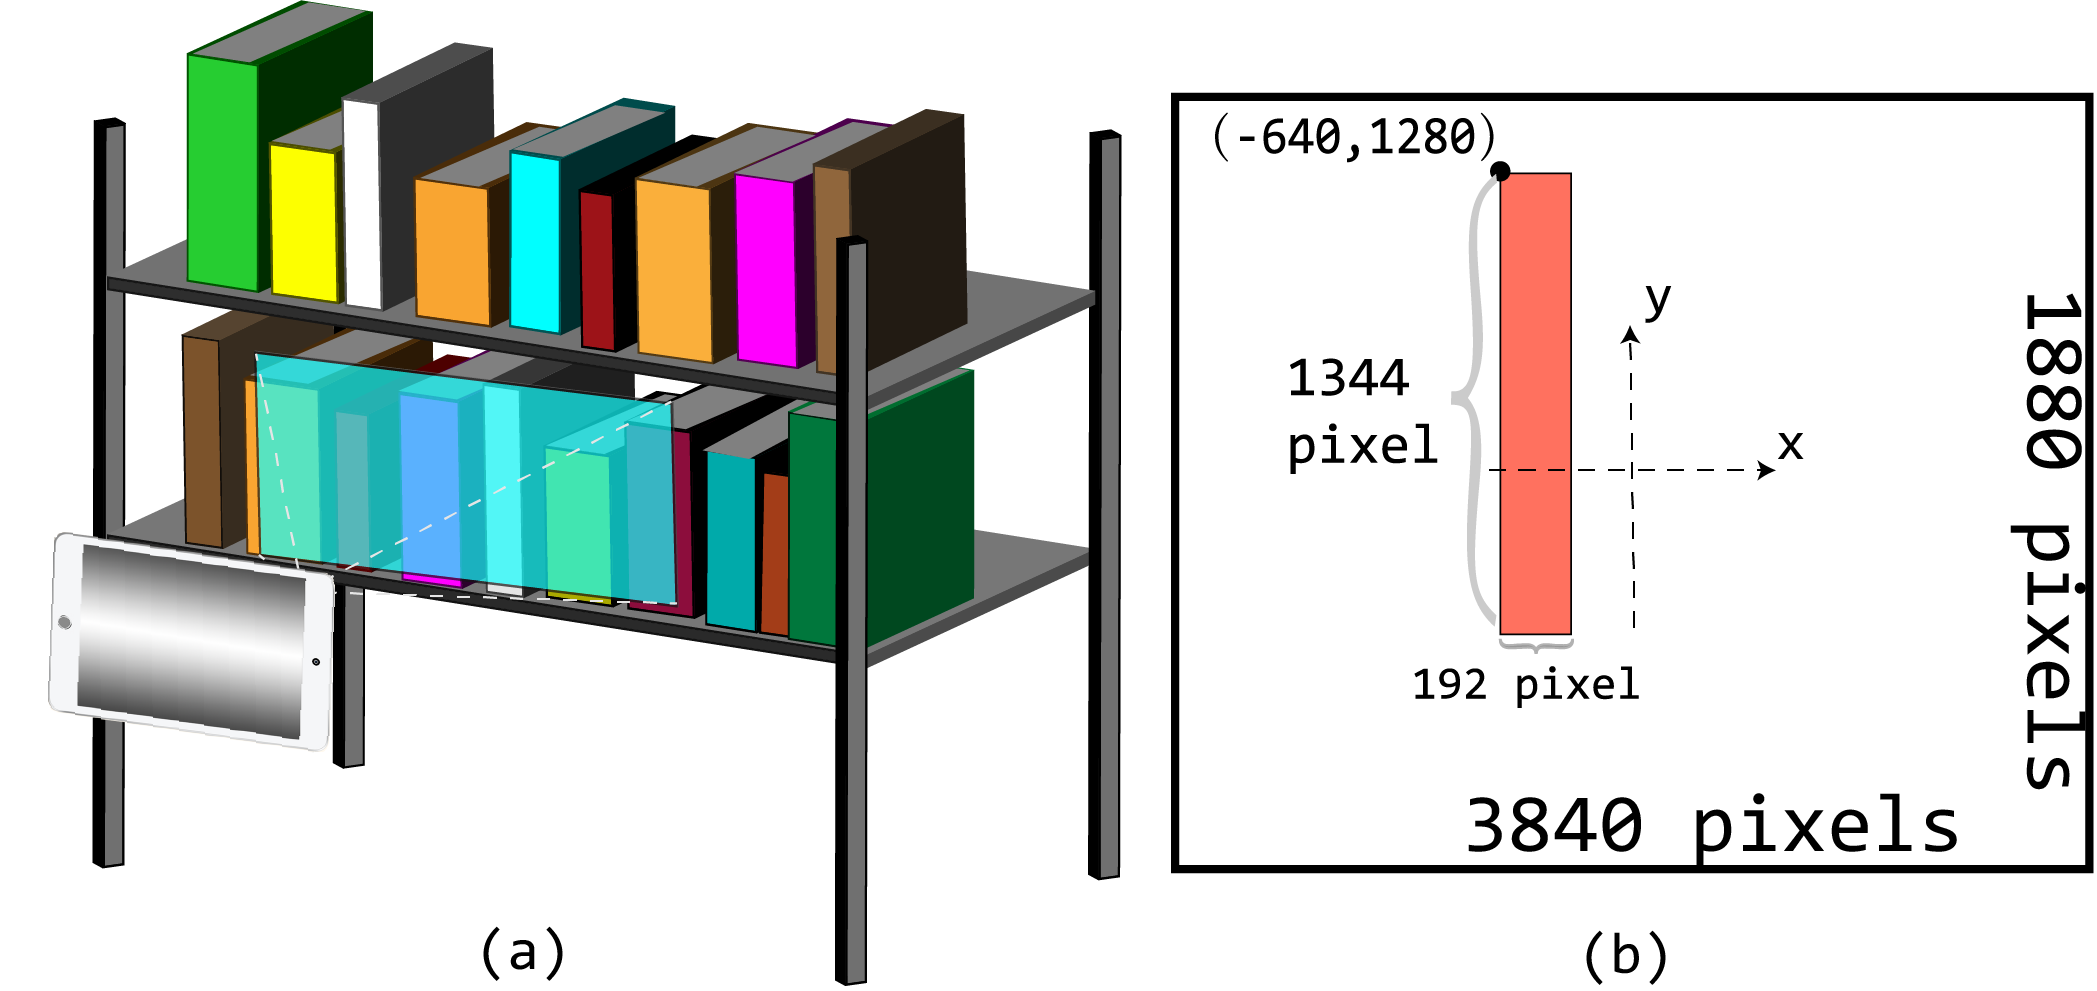
\includegraphics[width=\linewidth]{images/implementation_front.eps}
    \caption{
        %a,b,d三张图片没有在文中被引用,图片的整体描述不完整。
        The coordinate transformation algorithm. 
        (a): A mobile device is scanning the bookshelves.
        % (b): The top view of (a) showing the horizontal view angle $\alpha$,
        % where $d$ is the distance between the mobile device and the target books estimated by \textit{ARLayout},
        % and $x$ is the number of pixels horizontally.
        (b): A segmented book sample with the extracted position and size. %3840*1880
        % The coordinates of the top left corner of the book is (-640, 1280).
        % (d): Five blocks with recognized coffee names on a coffee menu.
    }
    \label{fig:implementation_front}
\end{figure}


\begin{figure*}[htp]
%\setlength{\abovecaptionskip}{0.05cm}
%\setlength{\belowcaptionskip}{-0.4cm}
    \centering
    \includegraphics[width=\linewidth]{images/implementation_network_deeplab.eps}
    \caption{
    The network illustration about how PaddleSeg is integrated into \textit{ARLayout}.
    We take DeepLab as an example, one of the key modules of PaddleSeg.
    The encoder module encodes multi-scale contextual information by
    applying atrous convolution at multiple scales, while the simple yet effective decoder
    module refines the segmentation results along object boundaries.
    }
    \label{fig:implementation_network_deeplab}
\end{figure*}


\subsection{Database}

We create a large database on the server for
three application scenarios that
require real-time information feedback~\cite{Mcauley2015, He2016}.
% Some of this data is in the scenario itself, such as the title of the book, the name of the coffee, the price, and some of it is not in the scenario, but is related to the objects in the scenario, such as the book’s evaluation, the composition of the coffee.
The database contains extra information of different dimentions, including books' ratings, 
coffees' ingredients, or eyeshadows' recommended schemes.
The mobile device can access the database and provides visual presentations for augmented information in realtime.
% providing visual presentations or personalized recommendations by accessing the database in realtime.

% \textbf{Global Book Database}
% A database of more than 2 million books is created on the server, making it easy to quickly find the ISBN, title, author, author introduction, abstract, publisher, cover image, pages, prices, tags, ratings, reviews, etc.
% The dataset comes from jmcauley.ucsd.edu/data/Amazon/.

% The dataset comes from jmcauley.ucsd.edu/data/Amazon/, containing product reviews and metadata from Amazon, including 143.7 million reviews spanning May 1996 - July 2014. It includes reviews (ratings, text, helpfulness votes), product metadata (descriptions, category information, price, brand, and image features), and links (also viewed/also bought graphs).

% This means that we are only building a global database of books, but our application scenario is not limited to this. In similar application scenario, \textit{ARLayout} can also provide other data support through pattern matching algorithm. In other words, an interface for fast data import can be implemented in future work to meet the data service requirements of more scenarios. We will continue this topic in the Discussion section.

% \textbf{Coffee/Cosmetics Database}
% These two databases are created by the Web crawler, which crawled collection from well-known coffee, cosmetics brand website.
% For example, coffee data comes from Starbucks, including the coffee’s name, description, ingredients list, preview image, process introduction, while eyeshadow data mainly comes from Dior, including eyeshadow color, eye shape, location, use steps, tips, recommendations.

\subsection{Optical Character Recognition}


% In actual applications,
We find that the traditional OCR methods are not available for some complex scenarios,
e.g. slanted texts (\autoref{fig:implementation_ocr} (a)), %artistic fonts (\autoref{fig:implementation_ocr} (e)),
or different text alignments in different languages (\autoref{fig:implementation_ocr} (c) and (d)).
The English texts (\autoref{fig:implementation_ocr} (c)) are often aligned in a vertical direction,
while the Chinese book texts (\autoref{fig:implementation_ocr} (d)) are often horizontally aligned.

In our experiments,
we improve the traditional OCR method, following a language adaptive design~\cite{Ling2018},
to achieve a large amount of the text characters over massive targets in reality.
In the approach, the texts of a book can be calibrated first if they are slanted (\autoref{fig:implementation_ocr} (b)),
and the language of a book will be identified first to correct its alignment,
which make the OCR recognition much more robust and scalable in the applications in reality.

%\textbf{Augmented OCR Network for Specific Scenarios}.
%Augmented template recognition works well when the texts are aligned well,
%e.g. the menu in a coffee shop.
%In the process of text recognition,
%the recognition template and classifier can be created according to different scenarios adaptively,
%which can automatically classify any regular format
%and output the recognition result in a structured way.
%In this section, there are two regions need to be settled.
%
%Reference region: the region pixels with fixed positions and contents
%in different pictures was chosen as anchor points of the picture,
%which can be used for template matching and rectification,
%as shown in~\autoref{fig:implementation_ocr} (f).
%Identification region: as shown in~\autoref{fig:implementation_ocr} (g),
%a field in a picture that needs to be identified
%was named to form a ``Key: Value'' relationship for ``Field name:
%Identification area content'',
%used to structurally identify the text contents.
%%of the same position of the same layout picture in real scenario.


\subsection{Convolutional Neural Network}
% Image sent from the mobile devices contains several targets.
We use image segmentation to recognize targets that contains in the images sent from the mobile devices.
The segmented target image will be labelled and sent back to the mobile devices
which visualize the targets in AR.
% In the actua
% AR can effectively help users migrate augmented information scenario
% to real-world scenarios for observation.
% Therefore, we use image segmentation
% to help us segment and label the components from the image,
% and then visualize the individual components in AR devices.
% In the actual implementation process, we sequential used the following methods to implement this function.

% \begin{figure}[htp]
%     \centering
%     \includegraphics[width=\linewidth]{images/BFS.eps}
%     \caption{
%         % (a) and (b) illustrate the process of BFS. In this image, each time the BFS cuts out the spine of a book.
%         (a) is the original photograph.
%         (b) is a single BFS expansion based on the pixel RGB values.
%         % (c) , (d) and (e) present scenarios that will have an negative impact on the effect.
%         (c) has several books of similar color, if they are adjacent, and the gap is very small, it may be considered as the same book.
%         (d) has a line between light and shadow in a shot, which can cause a book to be cut in half in poor lighting conditions.
%         (e) has a book with a color gap in its spine, and in real scenario it is possible that only the white parts are cut out.
%     }
%     \label{fig:BFS}
% \end{figure}

% \textbf{Breadth First Search}
% The algorithm was originally used for spine recognition in library/bookstore scenario. It is based on a basic assumption: the pixels at the spine of the book are basically continuous in RGB value. Therefore, on the basis of OCR, we approximate extend each text area with BFS algorithm until the pixel color transition too large, as shown in~\autoref{fig:BFS} (a) and (b). To show this process more clearly here, we have high-pixelated an area of the image. In real scenario, pixels extend by a much smaller step size (about 20 pixels per step, or 1/10 the size of the image). In the image, the green bolded edge points represent the current starting point, and the green unbolded edge points represent the feasible points that asingle BFS extension will reach. And the red points, represents the expanded RGB changes too large point. After a single BFS, all green points with unbolded edges will serve as starting points for the next round of BFS, continuing to expand the spine, while the red points will be discarded. At the end of algorithm, all the padding is the spine of a book.
% But this algorithm only based on RGB value, thus it shows high constraints in the actual use on the scenario, including lighting, spine design, etc. As shown in~\autoref{fig:BFS} (c) , (d) and (e). In addition, the assumption itself has a strong limitation: many objects do not have regular color separation. This means that the same algorithm is difficult to apply to other scenarios. Therefore, in the final version, we adopted the method of automatic segmentation of neural network to meet the needs of more scenarios.

% \textbf{Convolutional Neural Network}.
To get a better result for various scenarios in real applications~\cite{Zhu2020},
we apply an CNN-based open-source platform named PaddleSeg~\cite{Liu2019,Liu2021a}
to do image segmentation and labelling,
which only requires to manually annotate labels for a small amount of
samples for training (less than 100 for each usage scenario in this paper).
PaddleSeg is one of the state-of-the-art deep learning models for semantic image segmentation,
where the goal is to assign semantic labels (e.g., person, dog, cat and so on)
to every pixel in the input image.
In PaddleSeg, DeepLab~\cite{Chen2018} is one of its key modules.
Therefore, we take DeepLab as an example to
illustrate how PaddleSeg is integrated into \textit{ARLayout},
as shown in~\autoref{fig:implementation_network_deeplab}.
The encoder module encodes multi-scale contextual information by
applying atrous convolution at multiple scales, while the simple yet effective decoder
module refines the segmentation results along object boundaries.

%The panoramic pictures we captured or the real-time video we recorded
%are input into one of the three CNN networks (the top left of \autoref{fig:implementation_network}),
%while the labelled samples are input into the second CNN network (the top right of \autoref{fig:implementation_network}).
%Finally, the


\subsection{Coordinates Consistency between Virtuality and Reality}

To guarantee that the positions of the targets in AR space are consistent with their real-world positions,
we design the coordinate transformation algorithm.
% This guarantees the virtual-world positions of targets consistent with their real-world position.
On the client-side, pictures taken by users are sent back to
the server for recognition  (\autoref{fig:implementation_front} (a)).
The server sends back JSON data indicating the 2-D coordinates of targets in each picture.
Whenever a picture is taken, we use ARKit to detect a possible plane
in front of the camera and compute the distance $d$ between the plane and the
camera with LiDAR Scanner~\cite{ARKit}.
If given an image with resolution of 3840*1880 (\autoref{fig:implementation_front} (b)),
a red book is recognized at (-640,1280) with width 192 pixels and height 1344 pixels.
Therefore, the red book's volume and position can be calculated by the ratio 
between pixel and the measurement of the real world.


\subsection{Small Multiples and Virtual Models}

Regarding the visualizations for augmented information,
the related data will be sent to the server and the client will
receive the processed data from the server.
We design some visual presentation components like bar charts, line charts,
word cloud and the ingredients graphs, etc.,
which can be selected and composed for different usage scenarios.

We also create a virtual translucent screen in the AR environment to
show those augmented information.
Besides, in the eyeshadow scenario, we create a virtual head model,
stylize the model's eyes with the selected eyeshadow color
to show the 3-D preview presentations for users to help them
get a better fitting.





